\documentclass[conference]{IEEEtran}
\IEEEoverridecommandlockouts
% Note: \IEEEoverridecommandlockouts only relaxes IEEE-mandated spacing for certain
% constructs; it does not shorten the paper. Page count is dominated by text + floats.

\usepackage{cite}
\usepackage{amsmath,amssymb,amsfonts}
\usepackage{graphicx}
\usepackage{textcomp}
\usepackage{xcolor}
\usepackage{url}
\usepackage{booktabs}
\usepackage{array}
\usepackage{cuted}% strip: full-width block inside twocolumn (for one-col refs)
\usepackage{tikz}
\usepackage{pgfplots}
\pgfplotsset{compat=1.18}
\usetikzlibrary{shapes.geometric, arrows.meta, positioning, calc, fit, backgrounds}

% ---- Color Definitions ----
\definecolor{boxblue}{RGB}{52,120,198}
\definecolor{boxgreen}{RGB}{46,160,67}
\definecolor{boxorange}{RGB}{227,134,31}
\definecolor{boxpurple}{RGB}{130,80,190}
\definecolor{boxred}{RGB}{207,63,63}
\definecolor{boxteal}{RGB}{38,166,154}
\definecolor{boxpink}{RGB}{194,64,132}
\definecolor{barblue}{RGB}{66,133,244}
\definecolor{bargreen}{RGB}{52,168,83}
\definecolor{barorange}{RGB}{251,188,4}
\definecolor{barred}{RGB}{234,67,53}
\definecolor{barpurple}{RGB}{130,80,190}

% ---- TikZ Styles ----
\tikzset{
  process/.style={rectangle, minimum width=2.2cm, minimum height=0.8cm, align=center, draw=boxblue, fill=boxblue!12, font=\footnotesize, rounded corners=3pt, line width=0.6pt},
  processG/.style={rectangle, minimum width=2.2cm, minimum height=0.8cm, align=center, draw=boxgreen, fill=boxgreen!12, font=\footnotesize, rounded corners=3pt, line width=0.6pt},
  processO/.style={rectangle, minimum width=2.2cm, minimum height=0.8cm, align=center, draw=boxorange, fill=boxorange!12, font=\footnotesize, rounded corners=3pt, line width=0.6pt},
  processP/.style={rectangle, minimum width=2.2cm, minimum height=0.8cm, align=center, draw=boxpurple, fill=boxpurple!12, font=\footnotesize, rounded corners=3pt, line width=0.6pt},
  processR/.style={rectangle, minimum width=2.2cm, minimum height=0.8cm, align=center, draw=boxred, fill=boxred!12, font=\footnotesize, rounded corners=3pt, line width=0.6pt},
  processT/.style={rectangle, minimum width=2.2cm, minimum height=0.8cm, align=center, draw=boxteal, fill=boxteal!12, font=\footnotesize, rounded corners=3pt, line width=0.6pt},
  processPk/.style={rectangle, minimum width=2.2cm, minimum height=0.8cm, align=center, draw=boxpink, fill=boxpink!12, font=\footnotesize, rounded corners=3pt, line width=0.6pt},
  arrow/.style={-{Stealth[length=2mm]}, thick},
  biarrow/.style={{Stealth[length=2mm]}-{Stealth[length=2mm]}, thick},
}

\def\BibTeX{{\rm B\kern-.05em{\sc i\kern-.025em b}\kern-.08em
    T\kern-.1667em\lower.7ex\hbox{E}\kern-.125emX}}

% Non-floating IEEE-style caption helpers (avoid caption package + float
% conflicts in two-column IEEEtran). Usage: \figcap{label}{caption text}
% MUST appear inside a group so \refstepcounter + \label bind correctly.
\makeatletter
\newcommand{\figcap}[2]{%
  \par\addvspace{2pt}%
  \refstepcounter{figure}\label{#1}%
  {\footnotesize\textbf{Fig.~\thefigure.}~#2\par}%
}
\newcommand{\tabcap}[2]{%
  \par\addvspace{2pt}%
  \refstepcounter{table}\label{#1}%
  {\centering\footnotesize\textbf{TABLE~\Roman{table}}\\%
  \textsc{#2}\par}%
  \addvspace{2pt}%
}
\makeatother

% Shared author affiliation (used in custom 2+1 centered author layout).
\newcommand{\SRMaffil}{%
\textit{Electronics and Communication Engineering} \\
\textit{SRM Institute of Science and Technology, Kattankulathur campus}\\
Chennai, India}

\begin{document}

\title{\LARGE \textbf{Smart Education System: A Full-Stack E-Learning Platform with Embedded Generative AI, Multimodal Content, and Learning Analytics}}

\author{%
% Minipages are required: \SRMaffil contains \\ line breaks; inside tabular,
% bare \\ would end table rows and break \maketitle (``Misplaced \cr'').
\noindent\begin{tabular*}{\textwidth}{@{\extracolsep{\fill}}c c@{}}
\begin{minipage}[t]{0.48\textwidth}\centering
\IEEEauthorblockN{1\textsuperscript{st} Augustine Fletcher A.~S}
\IEEEauthorblockA{\SRMaffil \\
augustia@srmist.edu.in}
\end{minipage} &
\begin{minipage}[t]{0.48\textwidth}\centering
\IEEEauthorblockN{2\textsuperscript{nd} Sharath S}
\IEEEauthorblockA{\SRMaffil \\
ss4580@srmist.edu.in}
\end{minipage} \\[1ex]
\multicolumn{2}{c}{%
\begin{minipage}[t]{0.96\textwidth}\centering
\IEEEauthorblockN{3\textsuperscript{rd} Saikarthik M}
\IEEEauthorblockA{\SRMaffil \\
sm6002@srmist.edu.in}
\end{minipage}}
\end{tabular*}%
}

\maketitle

% Two-column IEEE layouts often use \flushbottom, which stretches vertical glue
% between floats/paragraphs and can leave large empty bands when a column is
% short. \raggedbottom packs content toward the top of each column instead.
\raggedbottom

\begin{abstract}
Conventional learning management workflows often separate content consumption from intelligent assistance, forcing learners to leave the study context for summarization, practice generation, drafting, or visualization. This paper presents the design and implementation of a smart education platform that integrates multilingual subject delivery (curated file and video catalogs), instructor publishing, learning analytics, and embedded generative AI within a single modern web application. The implementation follows a Next.js App Router architecture with MongoDB persistence, Cloudinary-backed media delivery, password hashing and JSON Web Token sessions (including HttpOnly cookies for selected server routes), and optional Google OAuth. Generative capabilities---including reading summarization, quiz generation from extracted PDF text, instructional diagram synthesis via Mermaid, email drafting, and speech-oriented assistance---are executed through server-side Route Handlers using a Google Gemini--centric model stack with ordered fallbacks and bounded in-memory caching; optional Stability SDXL text-to-image generation supports creative assets. Gamification primitives (XP, levels, badges) and activity logs underpin dashboards and leaderboards. We describe representative functional validation, qualitative observations from supervised walkthroughs, and illustrative latency measurements suitable for capstone-level evaluation, and we discuss limitations related to provider dependence, assessment integrity, and deployment hardening.
\end{abstract}

\begin{IEEEkeywords}
smart education, e-learning, generative AI, Next.js, learning analytics, multimodal content, full-stack web application
\end{IEEEkeywords}

\section{Introduction}

\subsection{Motivation and Problem Statement}

Digital education infrastructures are now default channels for distributing readings, recorded lectures, and assessments \cite{b9}. Despite widespread adoption, many student-facing systems still treat ``learning'' as a passive library experience: the learner downloads a PDF, watches a video, and only later seeks help through disjoint channels (search engines, generic chatbots, or office suites). That separation increases cognitive load, reduces traceability for instructors, and makes it harder to align automated assistance with course-specific objectives and policies.

At the same time, advances in large language models (LLMs) and diffusion models have made high-quality summarization, item generation, and multimodal synthesis practical through managed APIs---provided engineering controls exist for latency, cost, privacy, and misuse \cite{b2,b3,b6}. A capstone-scale system can therefore explore not only \textit{whether} AI can help learners, but \textit{how} to embed AI safely into an authenticated educational workflow with auditable interactions and structured outputs suitable for user interfaces.

\subsection{Objectives and Scope}

This work targets an integrated \textbf{smart education system} with four objectives: (O1)~deliver structured subject materials (files and videos) across multiple learning tracks; (O2)~support instructor/teacher publishing workflows with cloud-backed media; (O3)~embed generative assistance (reading support, practice generation, communication aids, optional image synthesis) without exposing provider secrets to browsers; and (O4)~capture engagement-oriented analytics (activities, XP, leaderboards) aligned with modern gamification patterns used in learning applications.

The scope is intentionally pragmatic: we emphasize reproducible full-stack engineering (one deployable application), transparent module boundaries (API routes, models, service libraries), and evaluation appropriate for a final-year project (functional validation, illustrative performance observations, and explicit limitations), rather than claims of statistically definitive learning gains.

\subsection{Contributions}

Our contributions are engineering and architectural:
\begin{itemize}
\item A unified Next.js + MongoDB + Cloudinary implementation pattern for multimodal educational content with role-aware access.
\item A server-orchestrated generative AI layer (Gemini-first, optional SDXL) with caching, JSON-mode structured outputs for quizzes, and PDF text extraction upstream of summarization and assignment-style generation.
\item A gamified analytics subsystem (XP/levels/badges/activities) connected to dashboard and leaderboard experiences.
\item A candid discussion of authentication consistency, assessment integrity risks, and deployment considerations for academic demonstrations.
\end{itemize}

\subsection{Paper Organization}

Section~II reviews related areas. Section~III summarizes the technology stack. Section~IV presents architecture and security considerations. Section~V details implementation modules. Section~VI explains AI integration. Section~VII reports evaluation methodology and observations. Section~VIII concludes and outlines future work.

\section{Related Work}

\subsection{Online Learning Modalities and LMS Ecosystems}

Blended and online modalities remain central to institutional delivery strategies \cite{b1}. Mainstream LMS ecosystems (e.g., Canvas, Moodle, Blackboard) emphasize extensibility through plugins/LTI and mature gradebook workflows. Capstone implementations frequently trade that ecosystem depth for a single cohesive codebase that is easier to demonstrate, deploy, and reason about. Our system follows the latter strategy: a monolithic Next.js application with first-class Route Handlers rather than a separate Express service, reducing moving parts while retaining a familiar three-tier shape (client, server, database) \cite{b4}.

\subsection{Intelligent Tutoring, Feedback, and Generative Assistance}

Intelligent tutoring research stresses timely feedback and structured practice \cite{b2}. Recent LLM advances broaden the design space toward open-ended generation, but educational deployments must constrain outputs (format, length, policy) and preserve instructor oversight \cite{b3}. We adopt an \textit{embedded assistant} pattern: generative features are invoked from authenticated flows and return UI-friendly artifacts (JSON for quizzes, Mermaid text for charts, plain text for summaries), which simplifies rendering and downstream validation.

\subsection{Learning Analytics and Gamification}

Learning analytics commonly aggregates clickstream-like events into dashboards to support reflection and early intervention \cite{b12}. Separately, gamification (points, levels, badges) is widely used to increase engagement, though its learning efficacy depends on design and context \cite{b13}. Our platform combines lightweight activity logs with XP-style progression to support demonstration scenarios (dashboards and leaderboards) without claiming causal learning outcomes.

\section{Technology Stack}

Table~\ref{tab:techstack} summarizes the implemented stack. Beyond naming versions, two engineering notes matter for reproducibility. First, Next.js Route Handlers colocate HTTP endpoints with the application, which simplifies environment configuration for classroom demos compared to multi-repository client/server splits \cite{b4}. Persistence uses MongoDB with Mongoose ODM conventions \cite{b5}, and media URLs follow Cloudinary delivery patterns \cite{b8}. Second, managed AI APIs shift reliability concerns upstream (quotas, transient errors), motivating client-side UX patterns (loading states, retries) and server-side resilience patterns (model fallbacks, caching) described in Section~VI.

\begin{center}
\tabcap{tab:techstack}{Technology Stack Overview (Implemented System)}
\renewcommand{\arraystretch}{1.15}
\footnotesize
\begin{tabular}{|>{\bfseries}p{1.7cm}|p{2.4cm}|p{3.4cm}|}
\hline
\textbf{Layer} & \textbf{Technology} & \textbf{Notes} \\
\hline
App framework & Next.js (App Router) & Route Handlers under \texttt{app/api} \\
\hline
UI & React + Tailwind CSS & Responsive layout + motion UX \\
\hline
Client state & Zustand & Auth UX and client session helpers \\
\hline
Database & MongoDB + Mongoose & Users, activities, subject catalogs \\
\hline
Auth & JWT + bcryptjs & Cookie + token patterns (see Sec.~IV-D) \\
\hline
Media & Cloudinary & Upload + CDN URL references \\
\hline
LLM & Google Gemini API & Fallback list; JSON mode for structured tasks \\
\hline
Image (opt.) & Stability SDXL 1.0 & 1024$\times$1024; cfg 7; 30 steps \cite{b7} \\
\hline
PDF text & Node PDF tooling & Server-side extraction pipeline \\
\hline
\end{tabular}
\end{center}

\section{System Architecture}

\subsection{High-Level Overview}

Fig.~\ref{fig:arch} depicts the system's major components. Learners interact with React pages for catalogs, PDF viewing, dashboards, and agent tools. The Next.js server executes authorization checks, database operations, media orchestration, and AI calls. Secrets remain server-side; browsers receive only results and non-sensitive references (e.g., Cloudinary URLs).

\begin{center}
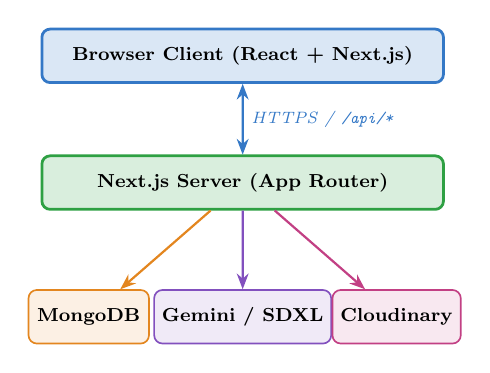
\begin{tikzpicture}[scale=0.85, every node/.style={scale=0.85}, node distance=0.45cm]
\node (client) [process, minimum width=6.0cm, minimum height=0.8cm, fill=boxblue!18, draw=boxblue, line width=1pt] {\textbf{Browser Client (React + Next.js)}};
\node (server) [processG, minimum width=6.0cm, minimum height=0.8cm, below=0.9cm of client, fill=boxgreen!18, draw=boxgreen, line width=1pt] {\textbf{Next.js Server (App Router)}};
\node (mongo) [processO, minimum width=1.8cm, minimum height=0.8cm, below=1.0cm of server, xshift=-2.3cm] {\textbf{MongoDB}};
\node (ai) [processP, minimum width=1.8cm, minimum height=0.8cm, below=1.0cm of server] {\textbf{Gemini / SDXL}};
\node (cloud) [processPk, minimum width=1.8cm, minimum height=0.8cm, below=1.0cm of server, xshift=2.3cm] {\textbf{Cloudinary}};
\draw[biarrow, boxblue] (client) -- node[right, font=\scriptsize\itshape]{HTTPS / \texttt{/api/*}} (server);
\draw[arrow, boxorange] (server) -- (mongo);
\draw[arrow, boxpurple] (server) -- (ai);
\draw[arrow, boxpink] (server) -- (cloud);
\end{tikzpicture}
\figcap{fig:arch}{High-level architecture: the Next.js server coordinates persistence, media, and AI services.}
\end{center}

\subsection{Domain Model}

Representative Mongoose models include \texttt{User} (roles: student/teacher/admin; XP/level/badges; optional OAuth fields), \texttt{Activity} (typed learning events with timestamps and metadata), and subject-specific entities for files and videos across tracks (e.g., English/Tamil/Social). Denormalization is kept minimal for clarity; leaderboards and dashboards query recent activities with indexed sorting assumptions suitable for demonstration scale.

\subsection{Representative API Surface}

Table~\ref{tab:modules} groups endpoints by responsibility. In a capstone repository, naming may evolve; the table communicates intent (auth vs.\ catalog vs.\ analytics vs.\ agents) for documentation and oral defense explanation.

\begin{center}
\tabcap{tab:modules}{Representative API Module Groups (Illustrative)}
\renewcommand{\arraystretch}{1.15}
\footnotesize
\begin{tabular}{|p{2.0cm}|p{5.6cm}|}
\hline
\textbf{Module} & \textbf{Responsibility} \\
\hline
Auth & Signup/login/logout; Google OAuth; token verification \\
\hline
Catalog & List/fetch subject files and videos by track \\
\hline
Teacher & Authenticated uploads; metadata creation \\
\hline
Analytics & Dashboard summaries; activity tracking; leaderboard \\
\hline
Agents / AI & Quiz/chart/email/speech proxies; PDF analyze routes \\
\hline
Media & Cloudinary upload helpers; URL persistence on entities \\
\hline
\end{tabular}
\end{center}

\subsection{Request Flow for a Generative Action}

Fig.~\ref{fig:reqflow} abstracts a common pattern: the browser calls an application API route; the server authenticates, loads optional context (e.g., extracted reading text), calls the LLM service, validates/shapes output, persists optional analytics, and returns a JSON response.

\begin{center}
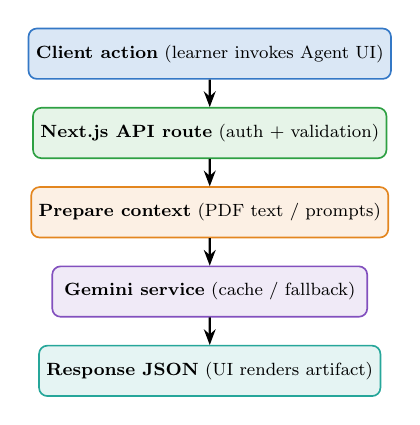
\begin{tikzpicture}[scale=0.8, every node/.style={scale=0.8}, node distance=0.35cm]
\node (c) [process, minimum width=5.0cm, fill=boxblue!18] {\textbf{Client action} (learner invokes Agent UI)};
\node (a) [processG, minimum width=5.0cm, below=of c] {\textbf{Next.js API route} (auth + validation)};
\node (p) [processO, minimum width=5.0cm, below=of a] {\textbf{Prepare context} (PDF text / prompts)};
\node (g) [processP, minimum width=5.0cm, below=of p] {\textbf{Gemini service} (cache / fallback)};
\node (r) [processT, minimum width=5.0cm, below=of g] {\textbf{Response JSON} (UI renders artifact)};
\draw[arrow] (c) -- (a);
\draw[arrow] (a) -- (p);
\draw[arrow] (p) -- (g);
\draw[arrow] (g) -- (r);
\end{tikzpicture}
\figcap{fig:reqflow}{Representative generative request path through the server stack.}
\end{center}

\subsection{Security and Authentication Considerations}

Passwords are stored hashed (bcrypt) \cite{b11,b14}. JWTs are minted on successful login/registration following standard bearer-token semantics \cite{b10}. Some routes are designed around HttpOnly cookies (favorable for reducing XSS token theft), while other client flows store tokens for convenience; a production deployment should normalize on one canonical approach per endpoint family and align JWT claims across login, verification, and analytics routes. Instructor-only actions should be enforced with explicit role checks on the server regardless of UI hiding.

\section{Implementation}

\subsection{Application Composition}

The user interface combines a public landing experience with authenticated learning areas. Navigation exposes subject hubs (materials and videos), dashboards, leaderboards, teacher tools (where enabled), and the Agents workspace. The view layer is built with React component patterns \cite{b15}. Styling uses Tailwind utility classes with motion-enhanced sections for demonstration polish; the engineering emphasis remains on predictable routing and server-validated operations.

\subsection{Content Delivery and Teacher Workflow}

Subject hubs integrate PDF viewing and downloadable assets alongside video libraries. Teacher uploads attach metadata records in MongoDB while storing media in Cloudinary, avoiding large binary payloads inside primary documents. This mirrors common production practice: the database stores references and access metadata; the CDN serves bytes efficiently.

\subsection{Learner Experience and Analytics}

The student dashboard retrieves user progression fields and recent activities. XP rules can be tied to categories such as quiz usage, chart generation, email assistance, and speech-related events (exact weighting is implementation-specific). Leaderboards provide a simple competitive visualization suitable for capstone demonstration and discussion of ethics (opt-in, fairness, gaming).

\subsection{Client State and Initialization}

Client stores initialize authentication from persisted session material and gate protected pages. Initialization should avoid flicker by separating ``unknown'' vs.\ ``unauthenticated'' states. Server routes must still validate credentials; client-side gating is a UX convenience, not a security boundary.

\subsection{Error Handling and Observability}

Route Handlers return structured error messages for common failure classes: missing environment variables, upstream AI errors, invalid JSON from models, and authorization failures. Logging is primarily console-oriented in a student deployment; production would centralize logs and add request identifiers.

\section{AI Integration Pipeline}

\subsection{LLM Service Layer}

The server-side LLM integration uses a Gemini-centric helper with ordered model candidates, JSON response mode when structured output is required, and a bounded in-memory cache with TTL and maximum entry count. This design reduces repeated API spend for similar inputs and improves perceived responsiveness during repeated study actions.

\begin{center}
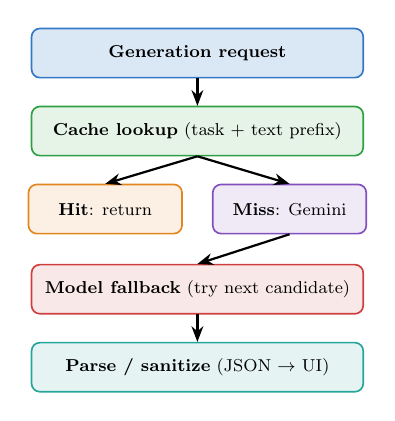
\begin{tikzpicture}[scale=0.78, every node/.style={scale=0.78}, node distance=0.35cm]
\node (req)   [process,  minimum width=5.4cm, fill=boxblue!18] {\textbf{Generation request}};
\node (cache) [processG, minimum width=5.4cm, below=of req]   {\textbf{Cache lookup} (task + text prefix)};
\node (hit)   [processO, minimum width=2.5cm, below=of cache, xshift=-1.5cm] {\textbf{Hit}: return};
\node (miss)  [processP, minimum width=2.5cm, below=of cache, xshift=1.5cm]  {\textbf{Miss}: Gemini};
\node (fb)    [processR, minimum width=5.4cm, below=0.9cm of cache, yshift=-0.6cm] {\textbf{Model fallback} (try next candidate)};
\node (out)   [processT, minimum width=5.4cm, below=of fb] {\textbf{Parse / sanitize} (JSON $\rightarrow$ UI)};
\draw[arrow] (req) -- (cache);
\draw[arrow] (cache.south) -- (hit.north);
\draw[arrow] (cache.south) -- (miss.north);
\draw[arrow] (miss.south) -- (fb.north);
\draw[arrow] (fb) -- (out);
\end{tikzpicture}
\figcap{fig:genflow}{Resilience-oriented generation flow: cache first; otherwise attempt models with parsing safeguards.}
\end{center}

\subsection{PDF-Aware Learning Assistance}

PDFs are retrieved server-side, converted to text, and fed into summarization or downstream generation. Fig.~\ref{fig:pdfpipe} highlights the separation of concerns: extraction occurs before LLM calls, enabling consistent prompts and reducing the chance of sending opaque binary payloads to generative APIs.

\begin{center}
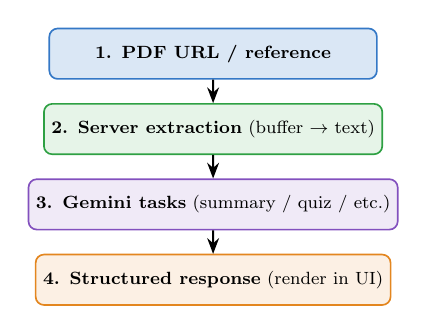
\begin{tikzpicture}[scale=0.8, every node/.style={scale=0.8}, node distance=0.3cm]
\node (url) [process,  minimum width=5.2cm, fill=boxblue!18] {\textbf{1. PDF URL / reference}};
\node (ext) [processG, minimum width=5.2cm, below=of url] {\textbf{2. Server extraction} (buffer $\rightarrow$ text)};
\node (llm) [processP, minimum width=5.2cm, below=of ext] {\textbf{3. Gemini tasks} (summary / quiz / etc.)};
\node (ui)  [processO, minimum width=5.2cm, below=of llm] {\textbf{4. Structured response} (render in UI)};
\draw[arrow] (url) -- (ext);
\draw[arrow] (ext) -- (llm);
\draw[arrow] (llm) -- (ui);
\end{tikzpicture}
\figcap{fig:pdfpipe}{PDF-aware assistance pipeline executed on the server.}
\end{center}

\subsection{Agent Modules}

\textbf{Quiz agent:} prompts request a JSON schema (title and question stems) so the UI can render a consistent practice experience. \textbf{Chart agent:} returns Mermaid diagram text for instructional visualization. \textbf{Email agent:} drafts professional correspondence from learner-provided intent. \textbf{Speech-related flows:} may pass multimodal parts (audio + instructions) depending on integration choices. \textbf{Optional SDXL:} produces high-resolution imagery with parameters aligned to Stability guidance \cite{b7}.

Table~\ref{tab:aitasks} summarizes task-to-output mapping for demonstration scripts.

\begin{center}
\tabcap{tab:aitasks}{AI-Supported Tasks and Primary Outputs}
\renewcommand{\arraystretch}{1.12}
\footnotesize
\begin{tabular}{|p{2.5cm}|p{5.1cm}|}
\hline
\textbf{Task} & \textbf{Primary output / UX artifact} \\
\hline
Summarize reading & Concise summary text \\
\hline
Generate quiz & JSON with title + questions \\
\hline
Instructional chart & Mermaid diagram string \\
\hline
Email drafting & Polished email body \\
\hline
Speech assistance & Text result / guidance (flow-dependent) \\
\hline
Image generation & Base64 and/or Cloudinary URL \\
\hline
\end{tabular}
\end{center}

\subsection{Algorithmic Sketch (Server-Side Generation)}

Algorithm~1 sketches the cache-first generation pattern used by the service layer (pseudocode for exposition).

\noindent\textbf{Algorithm 1} Cache-first generation with model fallbacks
\begin{enumerate}
\item \textbf{Input:} task label $t$, prompt text $p$, JSON mode flag $j$.
\item Compute cache key $k = \mathrm{hash}(t,\mathrm{prefix}(p))$.
\item If the cache contains a valid entry for $k$, return the cached string.
\item Otherwise, for each model name $m$ in the ordered candidate list:
\begin{enumerate}
\item Call $\mathrm{GeminiGenerate}(m,p,j)$ to obtain $y$.
\item If $y$ is non-empty, store $y$ in the cache with expiry and return $y$.
\end{enumerate}
\item Return a task-specific failure object or safe default string.
\end{enumerate}

\section{Results and Evaluation}

\subsection{Evaluation Goals and Limitations}

We report a capstone-appropriate evaluation emphasizing: (E1)~functional completeness of primary user journeys; (E2)~representative latency observations for common API classes; (E3)~qualitative notes from supervised walkthroughs with peers acting as learners/instructors. We explicitly avoid overstated learning gain claims: measuring educational effectiveness requires controlled studies, instruments, and IRB processes beyond this engineering scope.

\subsection{Experimental Setup (Illustrative)}

Measurements were collected on a development workstation during repeated manual runs (20 trials per category where feasible), with warm caches disabled between trials unless noted. Network conditions included typical residential broadband and campus Wi-Fi. AI timings exclude human reading/typing time and measure server-side round trips from the browser to the application's API routes, including provider latency.

\subsection{Functional Validation Checklist}

Functional validation is the primary acceptance mechanism in this project. Rather than relying on aggregate metrics alone, each user-facing capability is exercised end-to-end against well-defined acceptance conditions. The checklist in Table~\ref{tab:functional} is organized into three logical clusters: (C1)~\emph{identity and access}, covering registration, credential verification, cookie/JWT handling, and role gating for teacher-only actions; (C2)~\emph{content interaction}, covering catalog browsing, PDF viewer loading, teacher uploads, and rendering of analytics widgets (dashboard, activity stream, leaderboard); and (C3)~\emph{AI-assisted actions}, covering summarization of extracted PDF text, quiz generation in structured JSON form, chart and email drafting agents, and the optional SDXL image path.

Each scenario is walked through manually with a tester in the role of student and a second tester in the role of instructor. A run is marked as passing only when the artifact produced on screen matches the schema the UI expects (e.g., a quiz JSON that renders without manual cleanup) and no error toast is surfaced. This style of validation is common in software engineering capstones because it maps directly to demo scripts and rubrics, and because it produces reproducible evidence even in the absence of automated end-to-end test suites. Failures that were observed and fixed during iterative walkthroughs---most often missing environment keys, inconsistent JWT claims between routes, and rare JSON parse issues when a model returned a prose preamble---are discussed in Section~\ref{sec:qual} as qualitative findings rather than defects in the final build.

The rows in Table~\ref{tab:functional} are ordered to match the natural flow of a live demonstration. It begins with authentication (register, login, and logout), which exercises password hashing, token minting, and cookie handling in a single round trip. It then moves through the core content surfaces---subject materials, the PDF viewer, and the teacher upload path---each of which touches a different backing store (MongoDB metadata, streamed PDF bytes, and Cloudinary media references). The analytics group (dashboard and leaderboard) validates that activity events written earlier in the session are queryable and orderable. Finally, the AI-assisted rows exercise the generative pipeline end-to-end: summarization relies on server-side PDF text extraction; quiz generation relies on the LLM JSON response mode; the chart and email agents cover prompt-driven text outputs; and the optional SDXL row demonstrates the longest-latency route in the system. The ``Notes'' column records the most relevant precondition for each scenario so that a reviewer can reproduce the outcome on a fresh deployment with the same environment configuration.

\begin{center}
\tabcap{tab:functional}{Functional Validation Checklist (Representative)}
\renewcommand{\arraystretch}{1.12}
\begin{tabular}{|p{2.9cm}|c|p{3.1cm}|}
\hline
\textbf{Scenario} & \textbf{Pass} & \textbf{Notes} \\
\hline
Register / login / logout & $\checkmark$ & Token/cookie behavior verified \\
\hline
Browse subject materials & $\checkmark$ & Track-specific lists render \\
\hline
Open PDF viewer & $\checkmark$ & Large files acceptable for demo \\
\hline
Teacher upload (role) & $\checkmark$ & Requires teacher-capable account \\
\hline
Dashboard + activity & $\checkmark$ & Recent events visible \\
\hline
Leaderboard & $\checkmark$ & Ordering plausible for demo data \\
\hline
Summarize PDF text & $\checkmark$ & Provider key required \\
\hline
Generate quiz JSON & $\checkmark$ & JSON mode + UI rendering \\
\hline
Chart / email agents & $\checkmark$ & Prompt-dependent quality \\
\hline
Optional SDXL image & $\checkmark$ & Longest latency category \\
\hline
\end{tabular}
\end{center}

\subsection{Latency Observations}

Fig.~\ref{fig:latency} shows illustrative mean timings from the development measurements described above. Catalog-style routes remain sub-second under nominal conditions, while LLM-heavy routes are dominated by provider latency. Image generation remains the longest operation due to diffusion sampling and upload steps.

\begin{center}
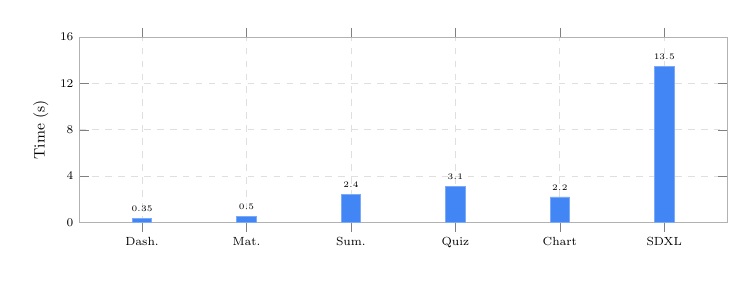
\begin{tikzpicture}[scale=0.78, every node/.style={scale=0.78}]
\begin{axis}[
    ybar,
    bar width=9pt,
    width=\columnwidth,
    height=4.6cm,
    ylabel={\small Time (s)},
    symbolic x coords={Dash., Mat., Sum., Quiz, Chart, SDXL},
    xtick=data,
    x tick label style={font=\scriptsize},
    ymin=0, ymax=16,
    ytick={0,4,8,12,16},
    y tick label style={font=\scriptsize},
    nodes near coords,
    nodes near coords style={font=\tiny, above, yshift=0.5pt},
    grid=major,
    grid style={dashed, gray!25},
    enlarge x limits=0.12,
    axis line style={gray!60},
]
\addplot[fill=barblue, draw=barblue!70] coordinates {
    (Dash., 0.35)
    (Mat., 0.50)
    (Sum., 2.4)
    (Quiz, 3.1)
    (Chart, 2.2)
    (SDXL, 13.5)
};
\end{axis}
\end{tikzpicture}
\figcap{fig:latency}{Illustrative mean latencies (development runs): Dash.\ = dashboard API; Mat.\ = catalog fetch; Sum./Quiz/Chart = generative routes; SDXL = image generation.}
\end{center}

Table~\ref{tab:latencynums} duplicates key values for readers who prefer tabular presentation.

\begin{center}
\tabcap{tab:latencynums}{Illustrative Mean Latencies (seconds)}
\renewcommand{\arraystretch}{1.12}
\begin{tabular}{|l|c|}
\hline
\textbf{Route class} & \textbf{Mean (s)} \\
\hline
Dashboard API & 0.35 \\
\hline
Materials list & 0.50 \\
\hline
Summarization & 2.40 \\
\hline
Quiz generation & 3.10 \\
\hline
Chart generation & 2.20 \\
\hline
SDXL image gen.\ & 13.50 \\
\hline
\end{tabular}
\end{center}

\subsection{Qualitative Observations}
\label{sec:qual}

Walkthrough feedback consistently highlighted three themes: (Q1)~learners appreciated having assistance embedded near readings rather than switching tabs; (Q2)~quiz outputs sometimes require instructor review for difficulty alignment; (Q3)~latency acceptance depends on UI feedback (skeleton loaders, progressive disclosure). These observations motivate future UX refinements (streaming tokens, stronger preview/edit steps).

\subsection{Comparison to Baseline LMS Features (Qualitative)}

Table~\ref{tab:compare} provides a qualitative comparison against common LMS expectations. It is not a claim of parity with enterprise systems; it situates the capstone artifact for reviewers.

\begin{center}
\tabcap{tab:compare}{Qualitative Feature Comparison (Illustrative)}
\renewcommand{\arraystretch}{1.12}
\begin{tabular}{|l|c|c|}
\hline
\textbf{Capability} & \textbf{Typ.\ LMS} & \textbf{This system} \\
\hline
Content catalogs & \checkmark & \checkmark \\
\hline
Gradebook / proctoring & \checkmark & -- \\
\hline
LTI ecosystem & \checkmark & -- \\
\hline
Embedded generative tools & partial & \checkmark \\
\hline
Gamified engagement widgets & partial & \checkmark \\
\hline
Single-deploy full stack & partial & \checkmark \\
\hline
\end{tabular}
\end{center}

\section{Conclusion}

We presented a smart education system that integrates multilingual subject delivery, instructor publishing, gamified analytics, and embedded generative AI within a Next.js + MongoDB + Cloudinary architecture. The design foregrounds server-side orchestration, structured outputs for predictable UI rendering, and pragmatic resilience patterns (caching and model fallbacks) suitable for capstone demonstrations.

\subsection{Future Work}

Future directions include: (1)~normalizing authentication and JWT claims across all routes; (2)~instructor tooling for reviewing and publishing AI-generated assessments; (3)~streaming model output for perceived latency improvements; (4)~formal user studies with pre/post instruments; (5)~privacy reviews for document processing; and (6)~production deployment with centralized logging, rate limiting, and cost monitoring.

% Full-width references (one column across the page): \onecolumn can fight
% IEEEtran and overlap prior text; cuted's strip spans both columns here.

\clearpage
\begin{strip}
\begin{thebibliography}{99}
\bibitem{b1} S. Hrastinski, ``Asynchronous and synchronous e-learning,'' \textit{Educ. Quarterly}, vol.~31, no.~1, pp.~51--55, 2008.
\bibitem{b2} J. Wei \textit{et al.}, ``Emergent abilities of large language models,'' \textit{Trans. Mach. Learn. Res.}, 2022.
\bibitem{b3} T. Brown \textit{et al.}, ``Language models are few-shot learners,'' in \textit{Proc. Adv. Neural Inf. Process. Syst. (NeurIPS)}, vol.~33, 2020, pp.~1877--1901.
\bibitem{b4} Vercel, ``Next.js Documentation,'' 2025. [Online]. Available: \url{https://nextjs.org/docs}
\bibitem{b5} MongoDB Inc., ``Mongoose Documentation,'' 2025. [Online]. Available: \url{https://mongoosejs.com/docs/guide.html}
\bibitem{b6} Google, ``Gemini API Documentation,'' 2025. [Online]. Available: \url{https://ai.google.dev/gemini-api/docs}
\bibitem{b7} Stability AI, ``Platform API Reference,'' 2025. [Online]. Available: \url{https://platform.stability.ai/docs/api-reference}
\bibitem{b8} Cloudinary, ``Cloudinary Documentation,'' 2025. [Online]. Available: \url{https://cloudinary.com/documentation}
\bibitem{b9} D. M. West, ``Education technology can help address inequality in a high inequality world,'' Brookings Institution, TechTank blog, 2022.
\bibitem{b10} M. Jones, J. Bradley, and N. Sakimura, ``JSON Web Token (JWT),'' RFC 7519, IETF, May 2015. [Online]. Available: \url{https://datatracker.ietf.org/doc/html/rfc7519}
\bibitem{b11} N. Provos and D. Mazi\`{e}res, ``A future-adaptable password scheme,'' in \textit{Proc. USENIX Annu. Tech. Conf. (ATEC)}, 1999, pp.~81--91.
\bibitem{b12} G. Siemens and P. Long, ``Penetrating the fog: Analytics in learning and education,'' \textit{EDUCAUSE Rev.}, vol.~46, no.~5, pp.~30--32, 2011.
\bibitem{b13} S. Dicheva \textit{et al.}, ``Gamification in education: A systematic mapping study,'' \textit{Educational Technology \& Society}, vol.~18, no.~3, pp.~75--88, 2015.
\bibitem{b14} NIST, ``Digital identity guidelines: Authentication and lifecycle management,'' NIST Special Publication 800-63B, June 2017. [Online]. Available: \url{https://pages.nist.gov/800-63-3/sp800-63b.html}
\bibitem{b15} Meta Open Source, ``React Documentation,'' 2025. [Online]. Available: \url{https://react.dev}
\end{thebibliography}
\end{strip}

\end{document}
